\documentclass[a4paper,twoside,openany]{book}
%twoside Specifies whether double or single sided output should be generated.
%openright/openany Makes chapters begin either only on right hand pages or on the next page available.
\usepackage{geometry}
\geometry{a4paper,top=3cm,bottom=3cm,left=3cm,right=3cm,heightrounded,bindingoffset=1cm}


\usepackage[italian, english]{babel}
\usepackage[T1]{fontenc}
\usepackage{lmodern}
\usepackage{color}
\usepackage{float}
\usepackage{graphicx}
\usepackage{amssymb}
\usepackage{amsmath}
\everymath{\displaystyle}
\usepackage{cancel}
\usepackage{booktabs}
\usepackage{multirow}
\usepackage{siunitx}
\usepackage{subcaption}
\usepackage{hyperref}
\usepackage{hyphenat}
\usepackage{verbatim}
\usepackage{chemformula}
\usepackage{color}
\definecolor{maroon(html/css)}{rgb}{0.5, 0.0, 0.0}
\usepackage{nicematrix}
\usepackage{rotating}

\begin{document}
	\begin{titlepage}
		\centering
		
\includegraphics[width=0.3\textwidth]{university}\\
		\bigskip
		{\Large
		{\scshape Università degli Studi di Milano Bicocca}\\
		{\scshape Dipartimento di Fisica}\\
		{\scshape "Giuseppe Occhialini"}\\
		\bigskip
		{\scshape Corso di Laurea Magistrale in Fisica}\\}
		Anno Accademico 2024/2025\\
		\bigskip
		{\hfill\vfill{\scshape \Huge{\textcolor{maroon(html/css)}{Characterization of \\a silicon detector}}}\\}
		{\vfill
		\[	\begin{array}{c}
			\mbox{Andrea Baiocco}\\
			\mbox{Giovanni Locatelli}\\
			\mbox{Gabriele Papasodaro}\\
			\mbox{Alberto Sala}
			\end{array}	\]}
	\end{titlepage}

\newpage
\null
\thispagestyle{empty}
\newpage

\pagenumbering{Roman}
\setcounter{page}{1}
\begin{center}\textbf{Summary}\\\end{center}
Study of the characteristics of a silicon ($\ch{Si}$PiN) detector and in particular the variation of energy resolution as a function of gain and shaping time by using a $^{55}\ch{Fe}$ radioactive source. Use the information thus obtained to study a multi-X source of ${241}Am$.

\begin{figure}[H]
\centering
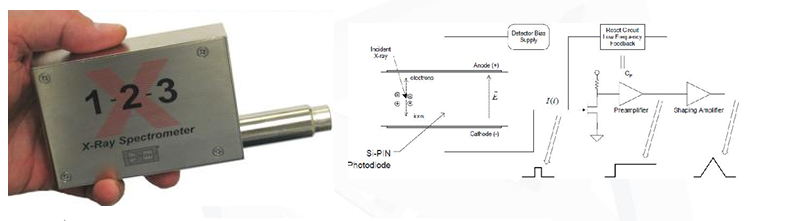
\includegraphics[width=1\textwidth, height=0.3\textwidth]{machine}
\caption{Machine design}
\label{schema}
\end{figure}

The design of the machine is the model showed in figure \ref {schema}. This model built for scientific studies allows you to change the gain and shaping time, , thus allowing us to characterize the energy resolution that we will measure.

The electronic chain described above allows the detected signal to be integrated and digitalised as shown in figure \ref{schema2}

\begin{figure}[H]
\centering
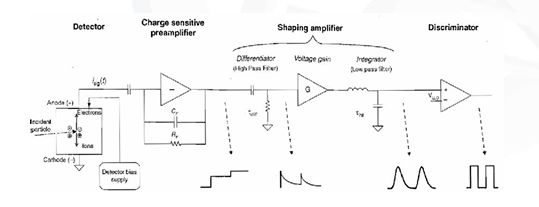
\includegraphics[width=0.8\textwidth, height=0.3\textwidth]{machine2}
\caption{Electronic design}
\label{schema2}
\end{figure}

The instrument can therefore be divided into 4 phases, the scintillator, a preamplifier, a shape amplifier and finally a discriminator.

\newpage
\null
\thispagestyle{empty}
\newpage

\pagenumbering{Roman}
\setcounter{page}{1}
\tableofcontents

\newpage
\null
\thispagestyle{empty}
\newpage

\pagenumbering{arabic}
\setcounter{page}{1}
\chapter{Instruments description}
	\section {Radioactive source}
\begin{itemize}
\item \ch{^{55}Fe}: This source decays by electron capture to an excited state of \ch{^{55}Mn}, which in turn decays to the ground state, emitting X-rays. The corresponding lines are the $k\beta$ line at 6.49 keV (decay from the third orbital to the S shell) and two $k\alpha$ lines at 5.898 and 5.887 keV, corresponding to the decay from the L shells (separated by spin-orbit interaction) to the S shell. The source has a half-life of 2.7 years, and given the activity 14 years ago, equal to 37 kBq, a current expected activity of 7.76 kBq can be derived.
\item \ch{^{241}Am}: This source decays mainly  into an excited state of  \ch{^{237}Np}, which then de-excites with gamma ray emission at 59.5 and 26.3 keV with various X-ray emissions. The most intense lines are: 11.87, 13.9, 16.9, 17.7, and 20.7 keV. This source also had an activity of 37 kBq 14 years ago and has a half-life of 432 years: its current activity will therefore be approximately 36.64 kBq. Being a multi-X source, it will have a spectrum with numerous peaks that simulates the spectrum of a plasma quite well, due to the impurities present within it.
\end{itemize}

In the experiment, the silicon detector "X-Ray Spectrometer 123" (\ref {schema}) was used. This is a PiN detector: it features a high-resistivity region inserted between the P and N junctions, with a thickness of approximately 300 $\mu$m, which allows for good resolution.

First, the detector must be calibrated. A \ch{^{55}Fe} source (described previously) was used, exploiting its two characteristic peaks at 5.9 keV and 6.5 keV. Next, in order to perform the measurements with the Americium source, it is necessary to find the optimal parameters to work with. The Gain and Shaping Time were varied to find the correct pair of values, also taking into account the associated dynamic range. Having taken all the necessary precautions, we can proceed to study the americium decay. To make the subsequent data analysis less laborious, during the experiment, some estimates were performed on paper, in order to have a draft of the results and thus be able to choose the optimal parameters to set during data collection.

\chapter{Data Analysis}
	\section{Calibration}
	\label{cal}
Performing measurements with the \ch{^{55}Fe} source yields the spectrum shown below (figure \ref{ferro})

Two peaks are therefore identified, corresponding to 5.9 keV and 6.5 keV. Since it was not possible to correctly distinguish the two peaks for the K-lines due to the short acquisition time of the measurements, only one peak at 5.9 keV was considered. A fit of the graph is performed at the two peaks to find the centroid and thus be able to perform the calibration, considering as the counting errors the error given by the Poissonian statistics, i.e., the square root of the counts themselves: 

\begin{figure}[H]
\centering
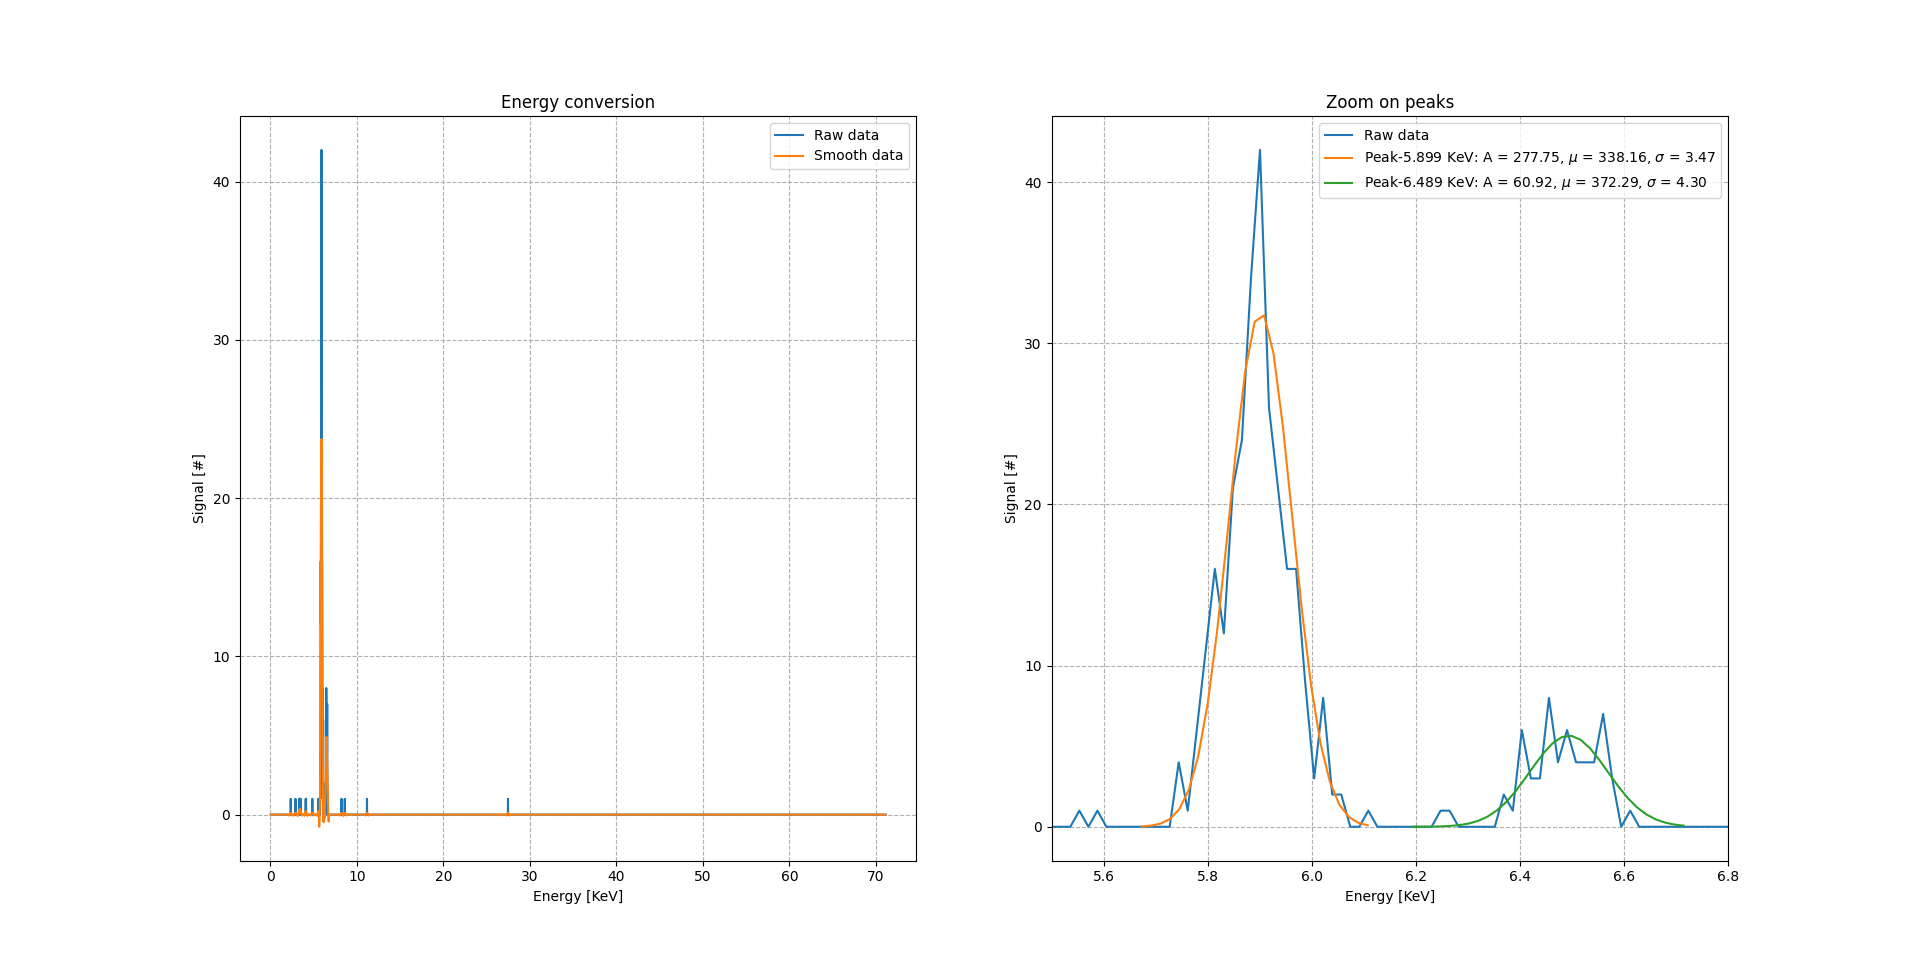
\includegraphics[width=0.9\textwidth, height=0.4\textwidth]{Calibrazione2}
\caption{Ferrum Spectrum}
\label{ferro}
\end{figure}

The following results are obtained for the centroids and the standard deviation:

\begin{table}[H]
\centering
\begin{tabular}{ccc}\hline
\textbf{Energy [keV]}&\textbf{Channel [Ch]}&\textbf{$\sigma$ [Ch]}\\\hline
5.899&338.16&3.74\\
6.489&372.29&4.30\\\hline
\end{tabular}
\caption{Energy, Channels parameters}
\label{Fe_peak}
\end{table}
\newpage
From which the following calibration is performed:

\begin{figure}[H]
\centering

\includegraphics[width=0.5\textwidth, height=0.4\textwidth]{Calibrazione}
\caption{Calibration}
\label{calibrazione}
\end{figure}

Obtaining the following result:

\begin{equation}
E [keV] = 1.735 \cdot 10^{-2} \cdot Ch + 3.371 \cdot 10^{-2}
\end{equation}

In particular, it is noted that the line does not pass exactly through the origin, but has an intercept that must be taken into account. Since there are two parameters for the line and two peaks used for calibration, it is not possible to perform a true $\chi^{2}$ test to verify the quality of the result. If the data had been acquired for a longer period of time, it would have been possible to separate the two peaks around 5.9 keV and thus perform a statistical test for calibration. 

Given monochromatic radiation, ideally one would like to obtain a Dirac Delta, but instead one obtains a Gaussian. Therefore, considering a Gaussian distribution, the energy resolution for the 5.9 keV peak is calculated using the relationship:

\begin{equation}
R_{energy} = \frac{FWHM}{H_{0}} = \frac{2.35\cdot\sigma}{H_{0}}
\label{resolution}
\end{equation}

Where $H_{0}$ is the centroid and the standard deviation obtained from the fit of the spectrum, obtaining:

\begin{equation}
R_{energy} = (2.36 \pm 0.01)\%
\label{fixed}
\end{equation}

The result obtained is compared with the results predicted by the Poisson statistics to check whether the detector is within the Poissonian limit for its intrinsic operation. Therefore, the energy resolution is required to satisfy the following relationship:

\begin{equation}
R_{energy} = \frac{2.35}{\sqrt{\epsilon}}
\end{equation}

where $\epsilon$ represents the centroid, or channel associated with our measurement. Therefore, requiring $\sigma = \sqrt{\epsilon}$  a resolution of (12.78$\pm$0.06)\% is achieved; the detector does not operate within the Poisson limit. At this point, we must introduce the Fano factor: a correction factor typically less than one, associated with the way the charges are generated within the detector, which allows us to correlate the variance obtained experimentally with that predicted by the Poisson statistic.

\begin{equation}
R_{energy} = 2.35\sqrt{\frac{F}{\epsilon}}
\end{equation}

The resulting Fano factor is $0.013\pm0.005$. In particular, this factor improves the instrument's resolution, that is, the Gaussian curve will be narrower than expected by the Poisson limit.

At this point, the detector's response to varying gain and shaping time is studied, trying to understand the optimal values for correct detector operation and studying how it varies with energy resolution. Gain represents the preamplifier's gain, i.e., how much the output signal is amplified, and can influence the energy resolution and dynamic range of the detector. Shaping time, on the other hand, represents the signal's formation time and impacts the duration and shape of the signal. In addition to energy resolution, this parameter can influence the signal-to-noise ratio.

A peculiar characteristic of the shaping time concerns the integration time of the signal. Because if we considered that for ong times, the energy of the peaks is measure, while for short times the arrival time of peaks is measured.\\

From this point on, we have considered three types of resolution. The first, which we will call `fixed', therefore considering a constant resolution previously calculated in the formula \ref{fixed}. The second and third modes, which we will instead call, albeit improperly, `nominal' and `statistical' resolution, where we will instead consider the equation \ref{resolution}. Therefore, for the left-hand side of the equation, we have developed a Python package capable of obtaining the FWHM resulting from a peak. For the right-hand side, we have applied a Gaussian fit as also shown in the \ref{cal} chapter, thus exploiting the non-monochromaticity of the radiation.

	\subsection{Detector Gain curve}
Initially, the shaping time is kept fixed at 16 $\mu$s and only the gain is varied (appendix \ref{app_gain}), calculating the energy resolution and fano factor for each of the obtained spectra, similarly to what was done above starting from the fit with Gaussians. 

The following trends are thus obtained:

\begin{table}[H]
\centering
\begin{tabular}{ccc}\hline
\textbf{File}&\textbf{Gain [dB]}&\textbf{Shaping Time [$\mu$s]}\\\hline
G1&4.986&16\\
G2&9.803&16\\
G3&29.938&16\\
G4&46.61&16\\
G5&72.829&16\\
G6&19.161&16\\
G7&46.61&16\\\hline
\end{tabular}
\caption{Gain range}
\label{range_gain}
\end{table}

\begin{figure}[H]
\centering
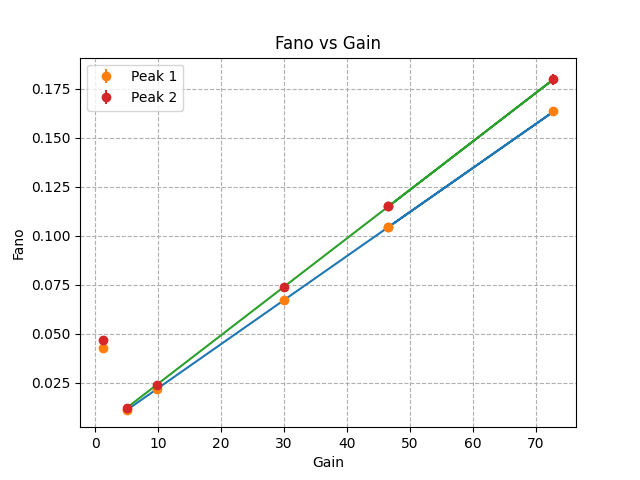
\includegraphics[width=0.4\textwidth, height=0.4\textwidth]{fano_gain_3}
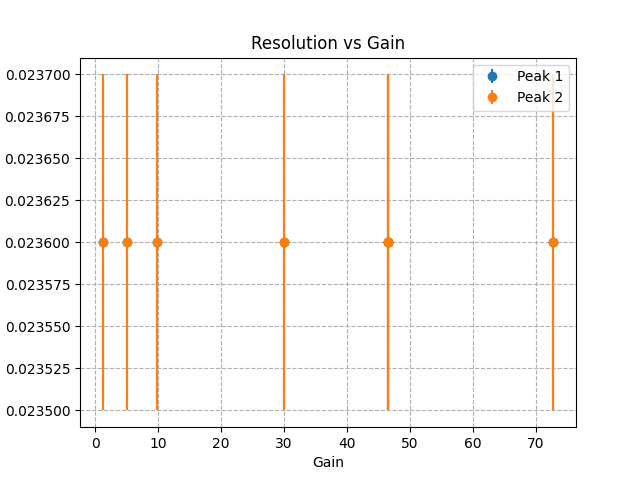
\includegraphics[width=0.4\textwidth, height=0.4\textwidth]{resolution_gain_3}
\caption{Fixed resolution}
\label{fixed_gain}
\end{figure}

\begin{figure}[H]
\centering
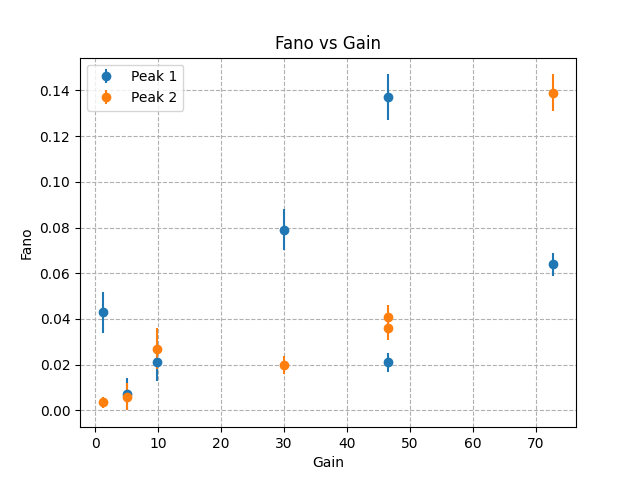
\includegraphics[width=0.4\textwidth, height=0.4\textwidth]{fano_gain_nom}
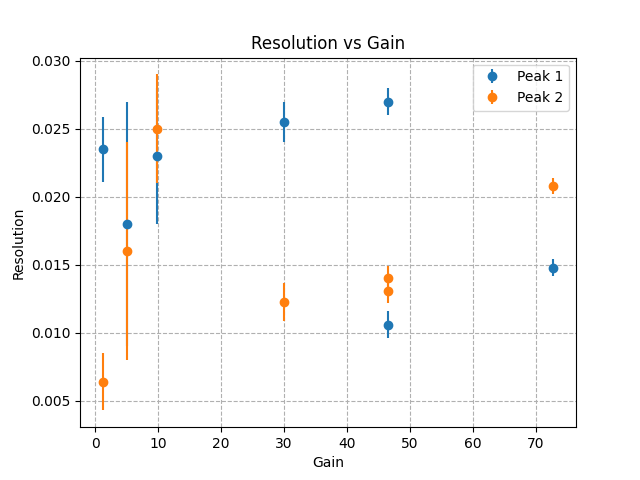
\includegraphics[width=0.4\textwidth, height=0.4\textwidth]{resolution_gain_nom}
\caption{Nominal resolution}
\label{nom_gain}
\end{figure}

\begin{figure}[H]
\centering
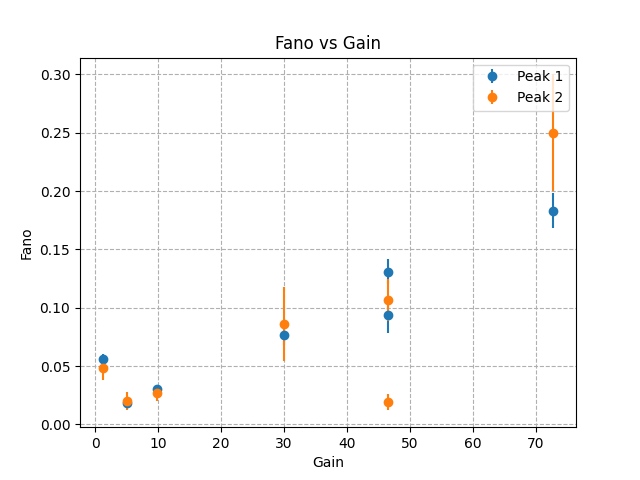
\includegraphics[width=0.4\textwidth, height=0.4\textwidth]{fano_gain_stat}
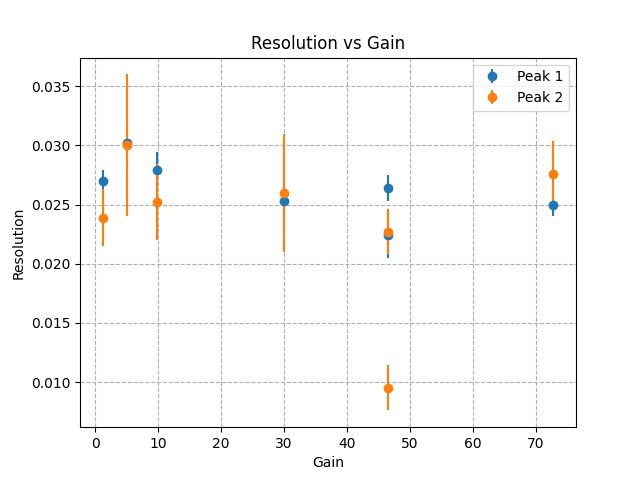
\includegraphics[width=0.4\textwidth, height=0.4\textwidth]{resolution_gain_stat}
\caption{Statistical resolution}
\label{stat_gain}
\end{figure}

	\subsection{Detector Shaping Time curve}
And then the measurements are repeated, by varying the shaping time and keeping the gain fixed at 15.335 dB (appendix \ref{app_sh}):

\begin{table}[H]
\centering
\begin{tabular}{ccc}\hline
\textbf{File}&\textbf{Gain [dB]}&\textbf{Shaping Time [$\mu$s]}\\\hline
live-data&15.335&32\\
S1&15.335&3.2\\
S2&15.335&5.6\\
S3&15.335&9.6\\
S4&15.335&16\\
S5&15.335&25.6\\
S6&15.335&44.8\\\hline
\end{tabular}
\caption{Gain range}
\label{range_gain}
\end{table}

\begin{figure}[H]
\centering
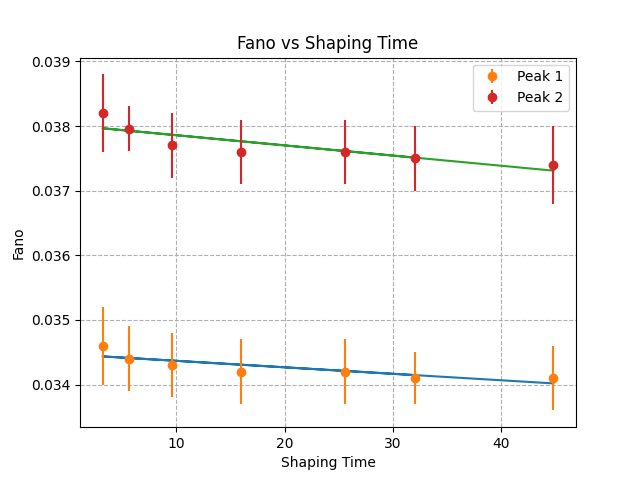
\includegraphics[width=0.4\textwidth, height=0.4\textwidth]{fano_shaping_3}
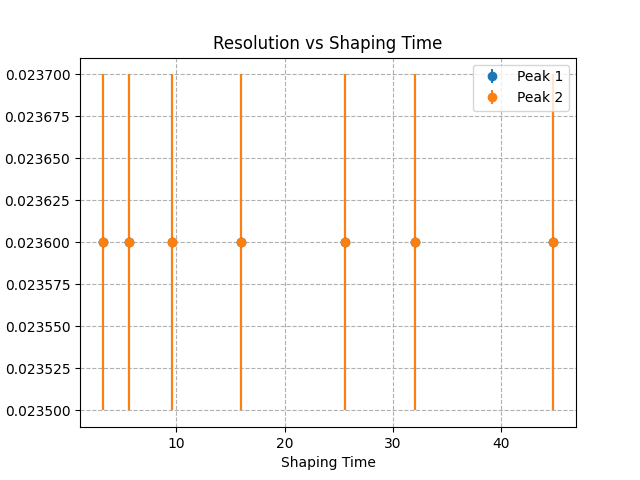
\includegraphics[width=0.4\textwidth, height=0.4\textwidth]{resolution_shaping_3}
\caption{Fixed resolution}
\label{fixed_sh}
\end{figure}

\begin{figure}[H]
\centering
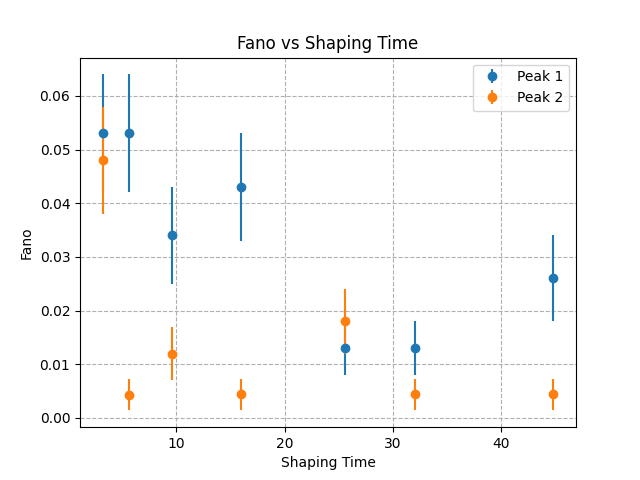
\includegraphics[width=0.4\textwidth, height=0.4\textwidth]{fano_shaping_nom}
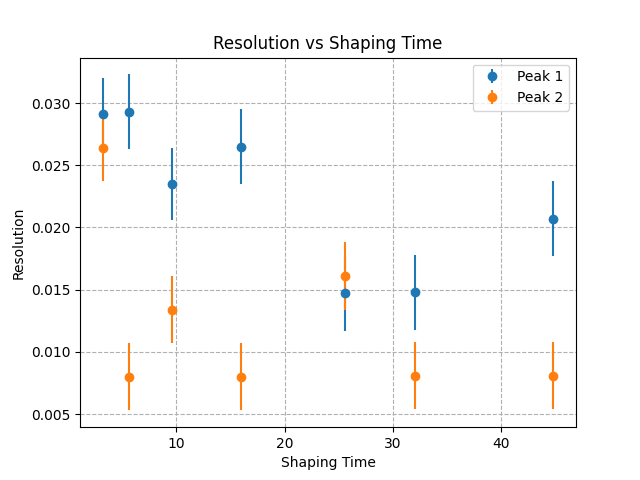
\includegraphics[width=0.4\textwidth, height=0.4\textwidth]{resolution_shaping_nom}
\caption{Nominal resolution}
\label{nom_sh}
\end{figure}

\begin{figure}[H]
\centering
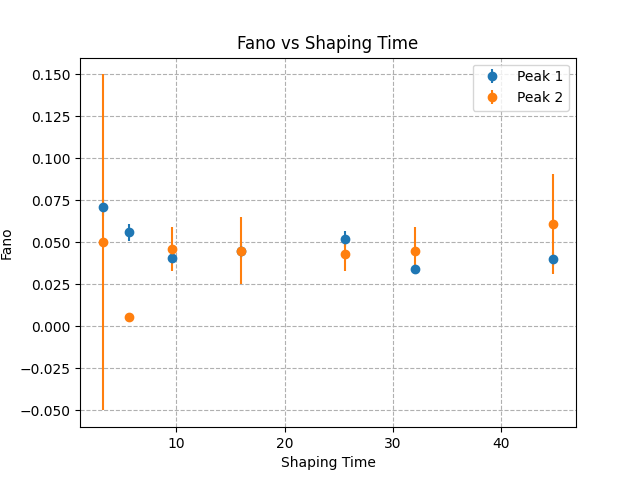
\includegraphics[width=0.4\textwidth, height=0.4\textwidth]{fano_shaping_stat}
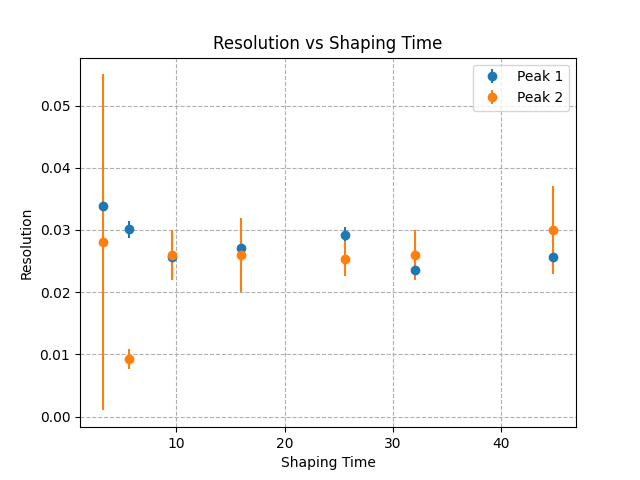
\includegraphics[width=0.4\textwidth, height=0.4\textwidth]{resolution_shaping_stat}
\caption{Statistical resolution}
\label{stat_sh}
\end{figure}

	\section{Conclusions on dynamic range}
Note how the resolution remains almost stable, in `statistical' mode, as the two parameters vary. In general, the lowest possible shaping time value will be chosen, in order to improve the rate capability, that is, the ability to identify and separate the greatest number of signals over time. Regarding the gain, another detail must be paid attention to: the dynamic range: This is the maximum range that can be represented on the x-axis for the detector. In fact, as the detector gain increases, the iron peak shifts toward increasingly larger channels, becoming lower and broader, thus increasing the standard deviation and keeping the energy resolution approximately stable. The problem lies in the possible calibration of the spectrum; in fact, the detector will be sensitive to increasingly lower energy ranges. This behavior must be related to what the detector wants to measure. In this case, the decay of an\ch{^{241}Am} source that has a visible peak at 60 keV. It was necessary to choose a gain that would allow this peak to be visualized.

The dynamic range provided by the graphs gave a maximum value in the channel of 4095. For the first two graphs, there are no problems fitting the peak, as can be easily verified starting from the calibration performed in the first part of the experiment, where the gain value was 16 dB.
The next spectrum is therefore calibrated starting from these results.

\begin{table}[H]
\centering
\begin{tabular}{c|c}
\textbf{Gain [dB]}&16\\
\textbf{Shaping Time [$\mu$s]}&32
\end{tabular}
\end{table}

	\section{Americio-241}
At this point, using the results obtained previously, that is, the correct value of shaping time and gain, we obtain the spectrum of \ch{^{241}Am}, measured for 30 minutes, figure \ref{americio}.

\begin{figure}[H]
\centering
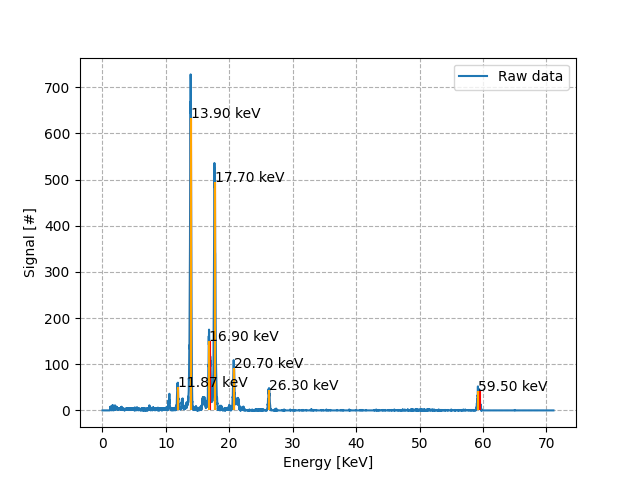
\includegraphics[width=0.6\textwidth, height=0.5\textwidth]{Americio1}
\caption{Americium Spectrum}
\label{americio}
\end{figure}

We get the peaks in the table that we are able to recognize (figure \ref{ameri}):
 
 \begin{figure}[H]
\centering
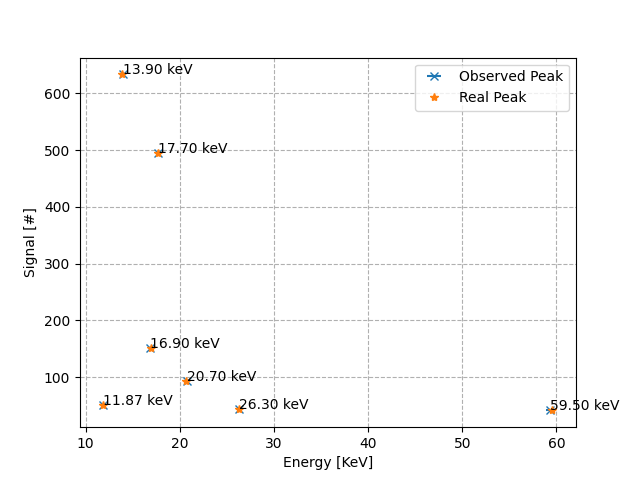
\includegraphics[width=0.6\textwidth, height=0.5\textwidth]{Americio2}
\caption{acceptance Americium peak}
\label{ameri}
\end{figure}
 
\begin{table}[H]
\centering
\begin{tabular}{cccc}\hline
\textbf{Real peak [keV]}&\textbf{Peak [keV]}&\textbf{$\sigma$ [keV]}&\textbf{Decay Radiation}\\\hline
11.87&11.87&0.08&X-ray \ch{^{237}Np}\\
13.9&13.92&0.09&X-ray \ch{^{237}Np}\\
16.9&16.84&0.11&X-ray \ch{^{237}Np}\\
17.7&17.69&0.11&X-ray \ch{^{237}Np}\\
20.7&20.71&0.13&X-ray \ch{^{237}Np}\\
26.3&26.25&0.17&$\gamma$-ray \ch{^{237}Np}\\
59.5&59.29&0.38&$\gamma$-ray \ch{^{237}Np}\\\hline
\end{tabular}
\caption{Energy peak}
\label{Am_peak}
\end{table}
 
 \appendix
\chapter{Gain}
\label{app_gain}

\begin{figure}[H]
\centering
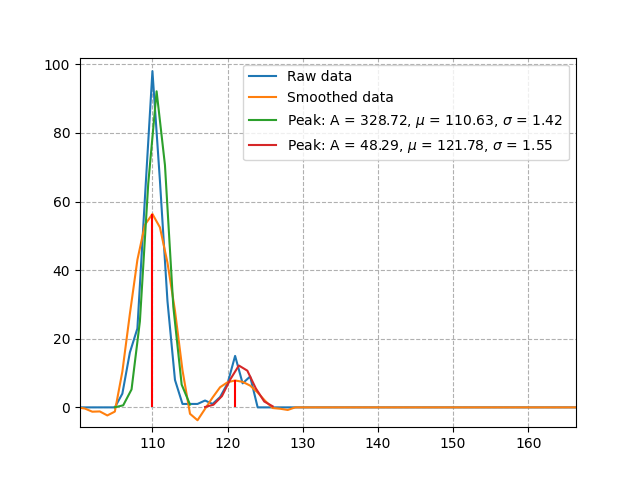
\includegraphics[width=0.3\textwidth, height=0.3\textwidth]{G1}
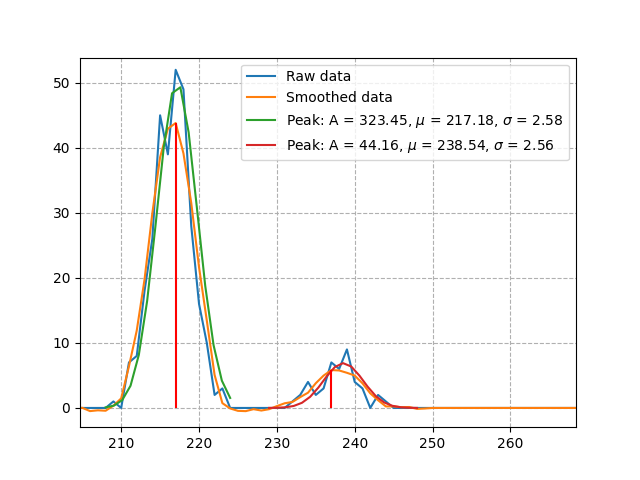
\includegraphics[width=0.3\textwidth, height=0.3\textwidth]{G2}
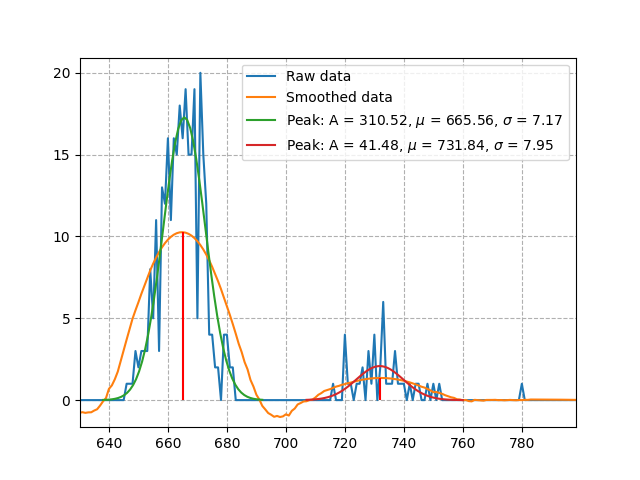
\includegraphics[width=0.3\textwidth, height=0.3\textwidth]{G3}
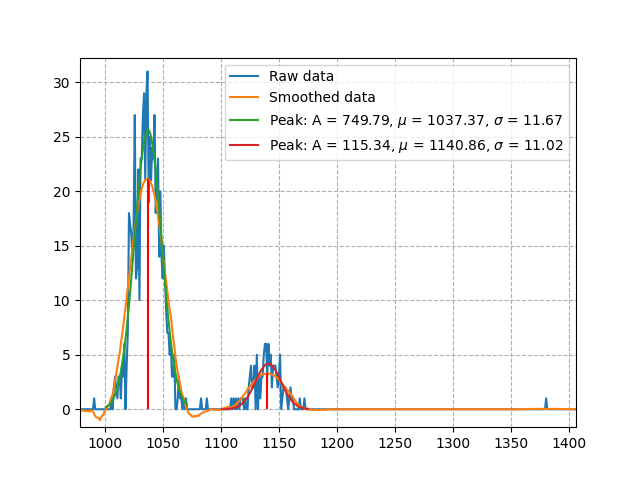
\includegraphics[width=0.3\textwidth, height=0.3\textwidth]{G4}
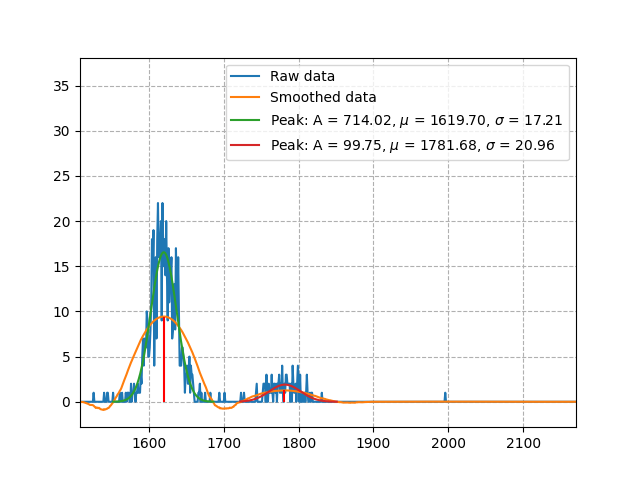
\includegraphics[width=0.3\textwidth, height=0.3\textwidth]{G5}
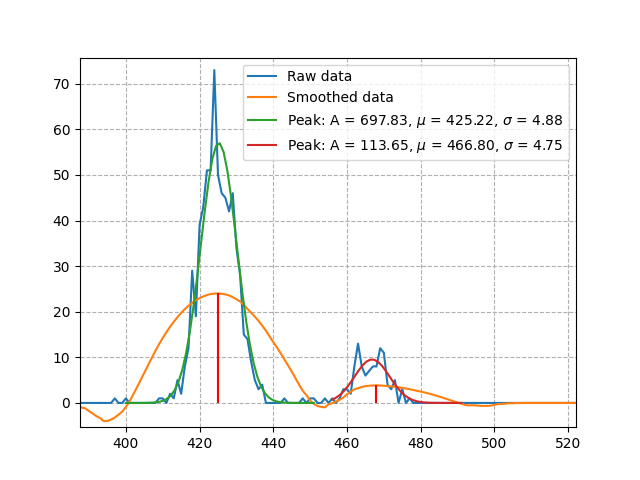
\includegraphics[width=0.3\textwidth, height=0.3\textwidth]{G6}
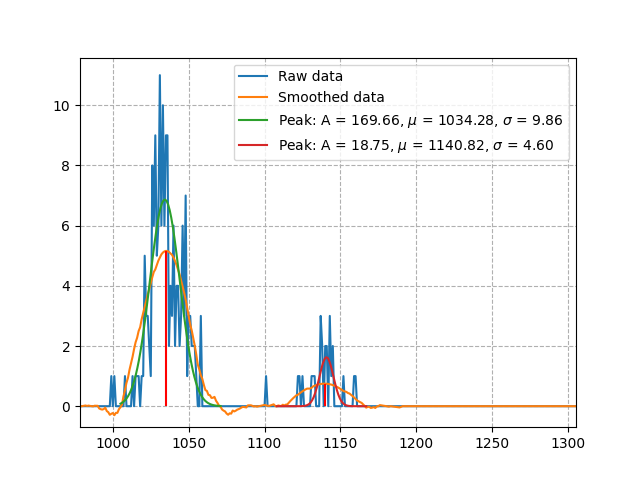
\includegraphics[width=0.3\textwidth, height=0.3\textwidth]{G7}
\caption{Appendix Gain}
\end{figure}

\chapter{Shaping Time}
\label{app_sh}

 \begin{figure}[H]
\centering
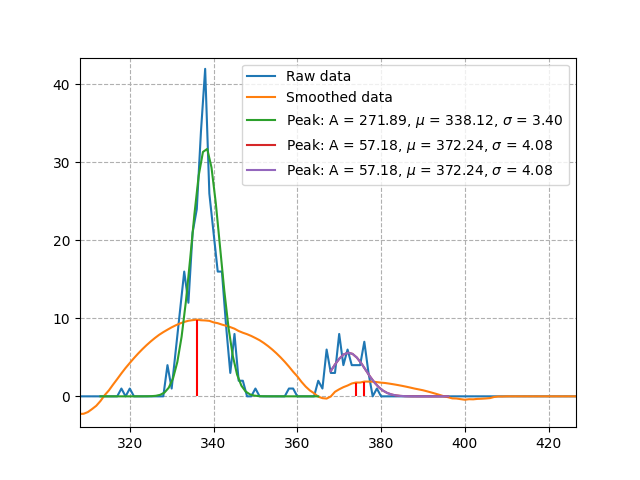
\includegraphics[width=0.3\textwidth, height=0.3\textwidth]{live_data}
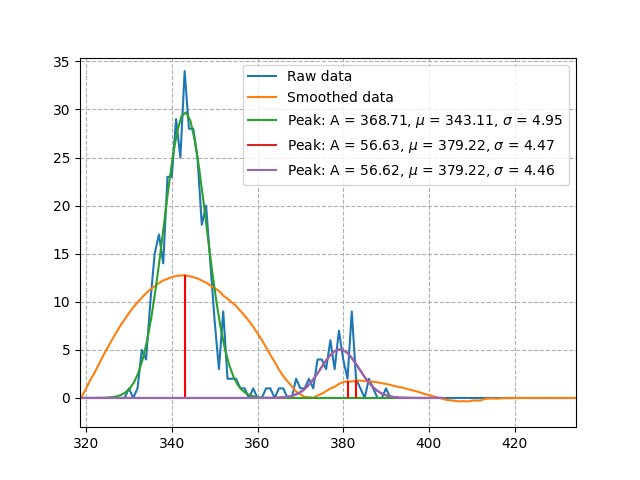
\includegraphics[width=0.3\textwidth, height=0.3\textwidth]{S1}
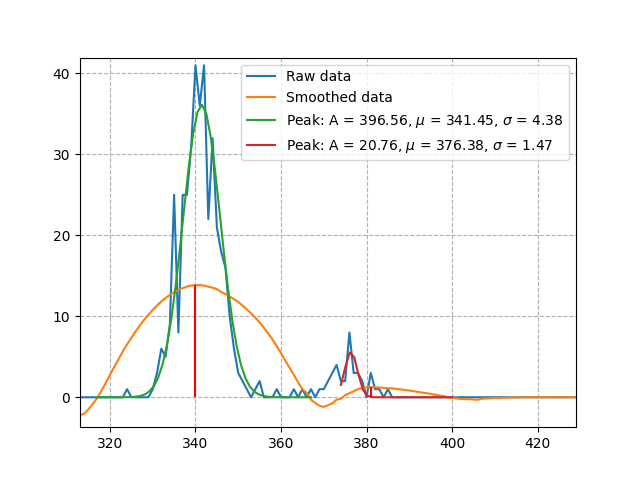
\includegraphics[width=0.3\textwidth, height=0.3\textwidth]{S2}
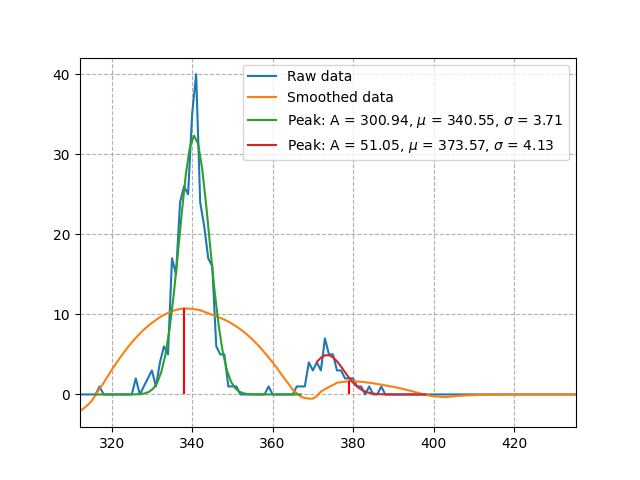
\includegraphics[width=0.3\textwidth, height=0.3\textwidth]{S3}
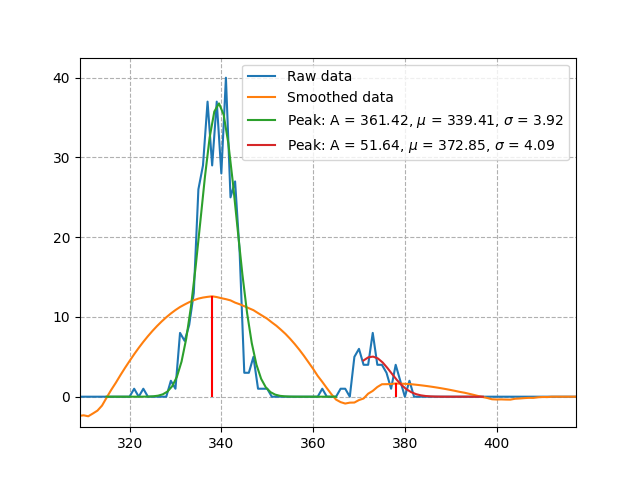
\includegraphics[width=0.3\textwidth, height=0.3\textwidth]{S4}
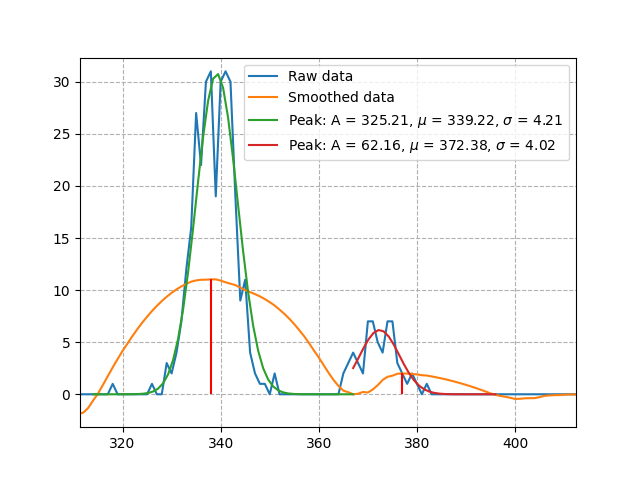
\includegraphics[width=0.3\textwidth, height=0.3\textwidth]{S5}
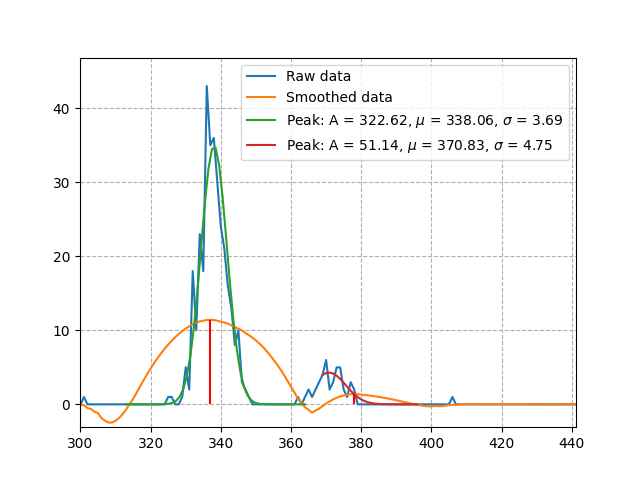
\includegraphics[width=0.3\textwidth, height=0.3\textwidth]{S6}
\caption{Appendix Shaping Time}
\end{figure}

\end{document}